\documentclass{standalone}
\usepackage{tikz}

\begin{document}
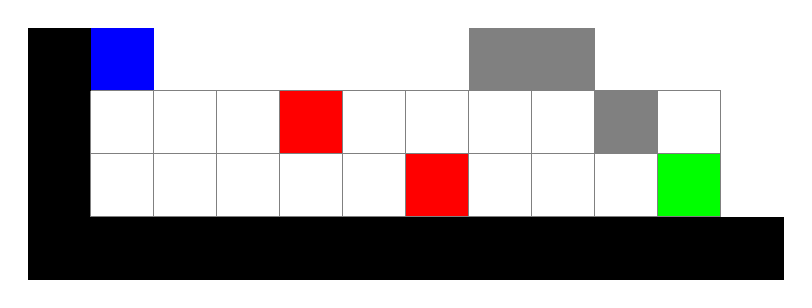
\begin{tikzpicture}[scale=0.8]

% Define colors for different elements
\definecolor{wall}{RGB}{0, 0, 0} % Black wall
\definecolor{path}{RGB}{255, 255, 255} % White path
\definecolor{agent}{RGB}{0, 0, 255} % Blue agent
\definecolor{switch}{RGB}{255, 0, 0} % Red switch
\definecolor{door}{RGB}{128, 128, 128} % Gray door
\definecolor{goal}{RGB}{0, 255, 0} % Green goal

% Draw the outer boundary (black wall)
\fill[wall] (0,0) rectangle (12,4);

% Draw the grid (white paths)
\foreach \x in {1,...,11} {
    \foreach \y in {1,...,3} {
        \fill[path] (\x,\y) rectangle ++(1,1);
    }
}

% Draw the agent (blue tile)
\fill[agent] (1,3) rectangle ++(1,1);

% Draw the red switches
\fill[switch] (4,2) rectangle ++(1,1); % First switch
\fill[switch] (6,1) rectangle ++(1,1); % Second switch

% Draw the gray doors
\fill[door] (7,3) rectangle ++(1,1); % First door
\fill[door] (8,3) rectangle ++(1,1); % Second door
\fill[door] (9,2) rectangle ++(1,1); % Third door

% Draw the green goal
\fill[goal] (10,1) rectangle ++(1,1);

% Optional: Add grid lines for clarity
\draw[step=1,help lines] (1,1) grid (11,3);

\end{tikzpicture}
\end{document}